%%% Dateikodierung: UTF-8
%%% äöüÄÖÜß  <-- keine deutschen Umlaute hier? UTF-faehigen Editor verwenden!

%%% Magic Comments zum Setzen der korrekten Parameter in kompatiblen IDEs
% !TeX encoding = utf8
% !TeX program = pdflatex 
% !TeX spellcheck = de_DE
% !BIB program = biber

\RequirePackage[utf8]{inputenc} % bei Verw. von lualatex oder xelatex entfernen!
\RequirePackage{hgbpdfa}        % Erzeugt ein PDF/A-2b-konformes Dokument

\documentclass[bachelor,german,smartquotes,proposal,alphabetic]{hgbthesis}
% Zulässige Optionen in [..]: 
%    Typ der Arbeit: 'diploma', 'master' (default), 'bachelor', 'internship'
%		 Zusätzlich für ein Thesis-Exposé: 'proposal' (für 'bachelor' und 'master')
%    Hauptsprache: 'german' (default), 'english'
%    Option zur Umwandlung in typografische Anführungszeichen: 'smartquotes'
%    APA Zitierstil: 'apa'
%%%-----------------------------------------------------------------------------


\graphicspath{{images/}}  % Verzeichnis mit Bildern und Grafiken
\logofile{logo}           % Logo-Datei: images/logo.pdf (kein Logo: \logofile{})
\bibliography{references} % Biblatex-Literaturdatei (references.bib)
\usepackage{hyperref}
\usepackage[acronym]{glossaries}

\makeglossaries

\newacronym{jvm}{JVM}{Java Virtual Machine}
\newacronym{vt}{VT}{Virtual Thread}
\newacronym{pt}{PT}{Plattform Thread}
\newacronym{ot}{OT}{Betriebssystem Thread}
\newacronym{sts}{STS}{StructuredTaskScope}                          % makeglossaries main in der cmd ausführen
\makeglossaries                           % makeglossaries muss dadurch nicht mehr in der cmd ausgeführt werden   

%%%-----------------------------------------------------------------------------
\begin{document}
%%%-----------------------------------------------------------------------------

%%%-----------------------------------------------------------------------------
% Angaben für die Titelei (Titelseite, Erklärung etc.)
%%%-----------------------------------------------------------------------------

% \title{Virtuelle Threads und strukturierte Nebenläufigkeitssteuerung in Java}
% \author{Gernot Hofbauer}
% \programname{Software Engineering}

% \programtype{Fachhochschul-Bachelorstudiengang}
% %\programtype{Fachhochschul-Masterstudiengang} % auswählen/editieren

% \placeofstudy{Hagenberg}
% \dateofsubmission{2024}{09}{26} % {YYYY}{MM}{DD}

% \advisor{FH-Prof. DI Johann Heinzelreiter} % optional
\pagenumbering{alph}                    % damit die Titelseite mit 'a' beginnt und links wieder richtig funktionieren
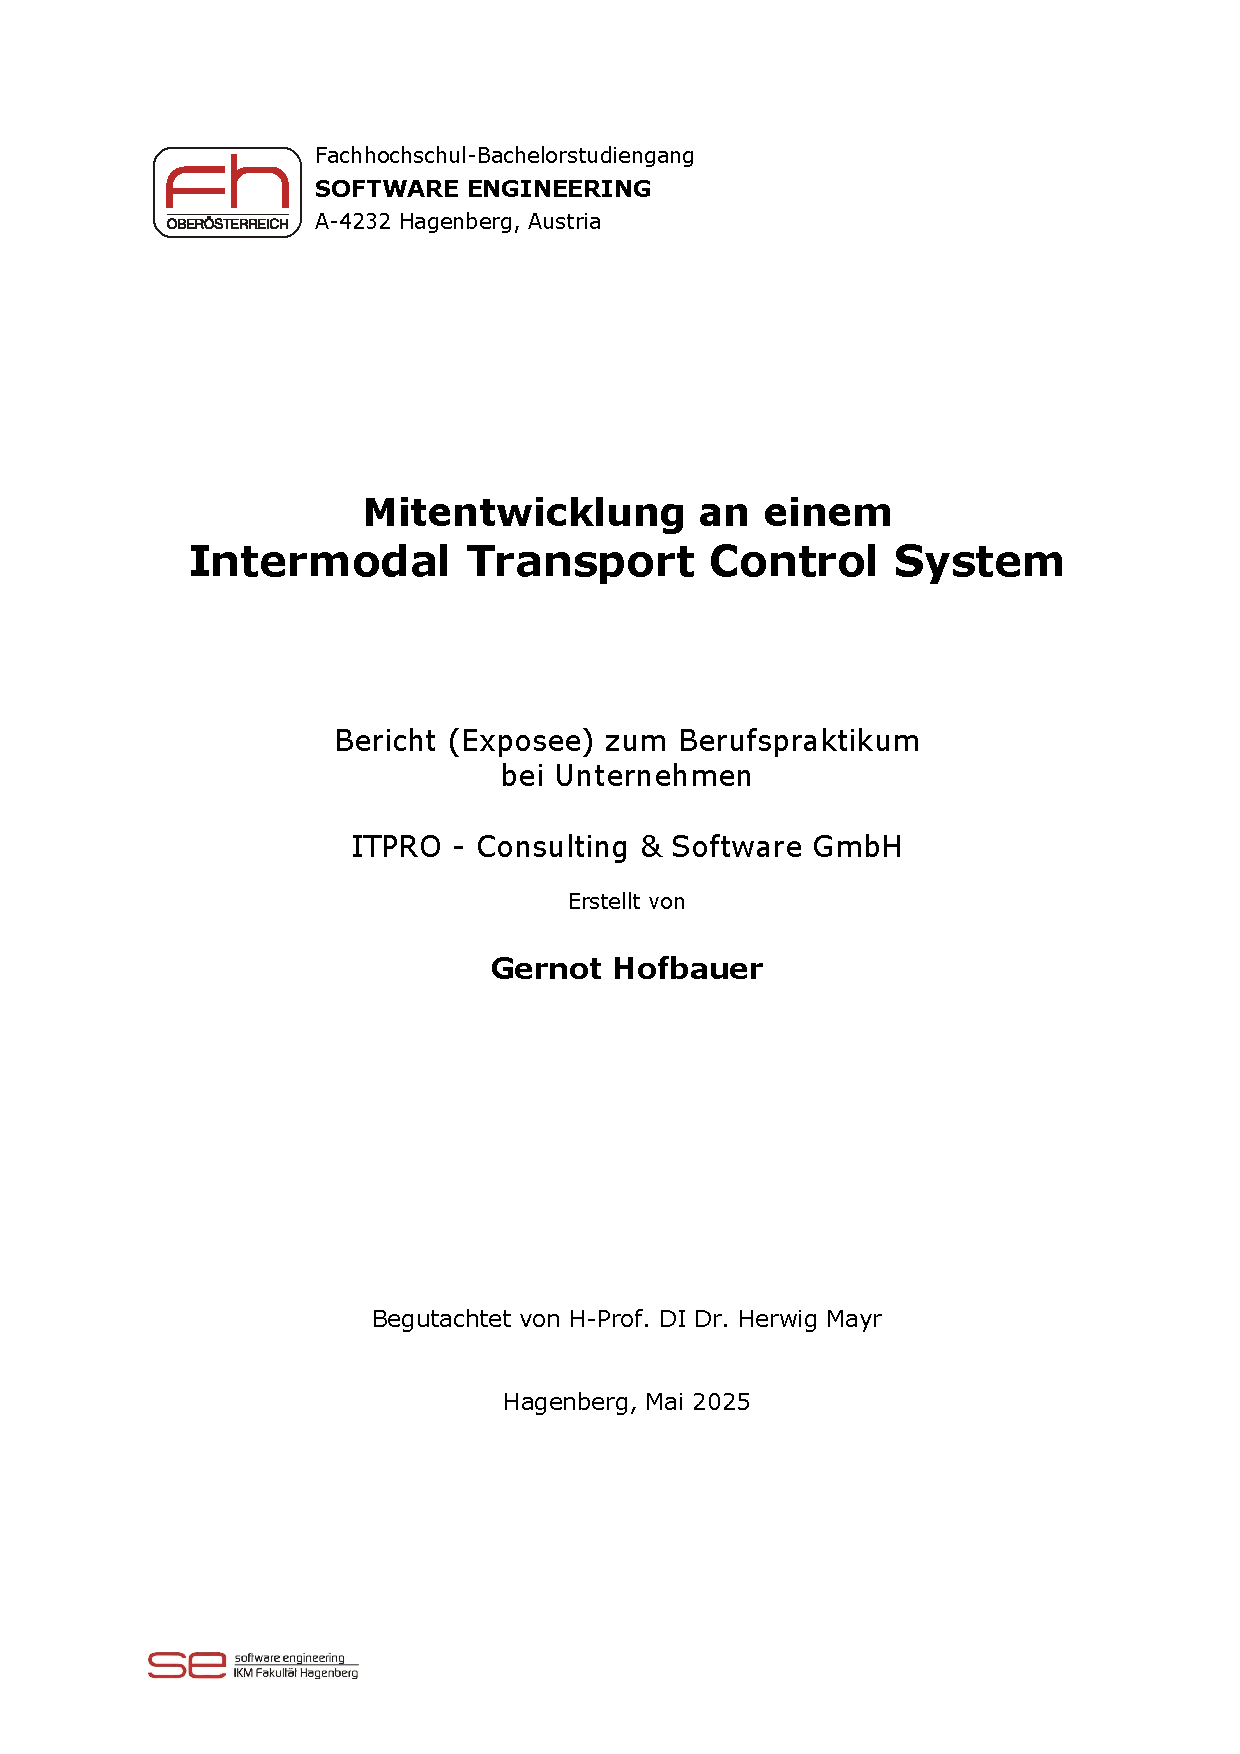
\includepdf[pages=-]{Titelblatt.pdf}

%%%-----------------------------------------------------------------------------
\frontmatter                                       % Titelei (röm. Seitenzahlen)
%%%-----------------------------------------------------------------------------

% \maketitle
\tableofcontents
\printglossary[type=\acronymtype,title=Akronyme]
%\chapter{Kurzfassung}

    Diese Bachelorarbeit befasst sich mit einigen Neuerungen von \emph{Project Loom} für Java. Es wird detailliert auf \emph{virtuelle Threads}, \emph{StructuredTaskScopes},
    die auch auf virtuellen Threads basieren
    und \emph{ScopedValues} eingegangen.
    Zu jeder dieser Technologien wird zunächst eine technische Übersicht geboten, bei der darauf eingegangen wird, inwiefern sie sich von den bereits bekannten Technologien unterscheiden.
    Darauf folgt eine eine Erklärung, wie sie in Java verwendet werden können, wobei einige Beispiele gezeigt werden. 
    Bei \texttt{StructuredTaskScopes} beinhaltet dies auch das Einbinden eigener Logik und Fehlerbehandlung durch Ableitung von der Basisklasse. Bei \texttt{ScopedValues} wird auch auf die Unterschiede zu \texttt{ThreadLocal} eingegangen. 
    Um eine besseren Vergleich zwischen den bekannten Technologien und den Neuerungen von Projekt Loom ziehen zu können, wird das Laufzeitverhalten eingehend analysiert. Dazu wurden sechs einfache Benchmarks,
    welche das Laufzeitverhalten untersuchen, erstellt und durchgeführt. Aufgrund von Schwierigkeiten
    beim Messen des Speicherverbrauchs wurde zu diesem Aspekt nur ein Test durchgeführt. Die Messergebnisse wurden ausführlich analysiert und interpretiert.
    Dabei wurde festgestellt, dass virtuelle Threads in in den meisten Fällen Plattform-Threads überlegen sind. Lediglich bei wenigen, stark rechenintensiven Aufgaben, ganz ohne blockierende Aufrufe, 
    sollten Plattform-Threads bevorzugt werden. Eine der größten Stärken von virtuellen Threads ist die Möglichkeit, in sehr großen Mengen, ohne viel Overhead erstellt zu werden. 
    Dadurch skalieren sie besser und sind leichtgewichtiger als Plattform-Threads.
    ScopedValues sind bei der Vererbung von Werten über Threads hinweg schneller als ThreadLocal und benötigen bei großen Mengen an Threads wesentlich weniger Speicher. 
    Sie können daher in Kombination mit virtuellen Threads sehr empfohlen werden. Die Wertabfrage selbst ist aber ein wenig langsamer als bei ThreadLocal.
    Im Gegensatz zu ThreadLocal sind ScopedValues nicht veränderbar und können somit nicht immer als Ersatz verwendet werden.
		
%\chapter{Abstract}

\begin{english}
Large Public Display Games place several specific design requirements. Such
games need to work equally well for just a few or several simultaneous users.
Also, entering, leaving, or joining a game in progress should be easily possible
without interrupting the game's flow. This bachelor (master) thesis focuses on
developing a game mechanics framework that supports the principle of smooth
transition gameplay. This framework will then be evaluated utilizing a prototype
implemented in a term project.
\end{english}
			


%%%-----------------------------------------------------------------------------
\mainmatter                             % Hauptteil (ab hier arab. Seitenzahlen)
%%%-----------------------------------------------------------------------------

\chapter{Exposé}

\section{Einleitung}

	% Der \emph{Deep Space 8K}%
	% \footnote{\url{https://ars.electronica.art/center/de/exhibitions/deepspace/}}
	% des Ars Electronica Centers in Linz bietet mit seiner $16 \times 9$~m
	% großen Projektionsfläche inklusive Positionstracking eine einzigartige
	% Möglichkeit, Computerspiele zu realisieren. Diese Spiele verwenden keine
	% klassischen Kontrollmechanismen wie Tastatur, Maus oder Gamepad sondern die
	% Spieler*innen selbst "steuern" die Inhalte mit ihren Bewegungen. Darüber
	% hinaus finden diese Spiele in einem halb-öffentlichen bis öffentlichen Raum
	% statt, wodurch sich die Bestimmung der Zielgruppe sowie die Anzahl der
	% spielenden Personen schwierig gestaltet. Diese Bachelorarbeit (Masterarbeit)
	% beleuchtet diese Problematik und stellt konkrete Lösungsvorschläge anhand
	% eines Beispiels dar.

	% Seit einigen Jahren Arbeitet Oracle an Möglichkeiten zur Verbesserung der Skalierbarkeit von Java-Anwendungen im Projekt "Loom".
	% Der Hauptansatz dieses Vorhabens ist die Einführung von virtuellen Threads, die von der JVM verwaltet werden. 
	% Diese Threads sind leichtgewichtiger als klassische Plattform Threads und können in größerer Anzahl erzeugt werden. 
	% In Kombination mit "Continuations" \cite{Continuations}, die es ermöglichen sollen, die Ausführung von Threads zu pausieren und fortzusetzen,
	% können so bestimmte Anwendungen mit hoher Nebenläufigkeit zukünftig effizienter gestaltet werden. Diese Bachelorarbeit 
	% beleuchtet diese Technologien und stellt die Neuerungen dem bereits Bekanntem gegenüber.

	Um den Abschluss des Fachhochschul-Bachelorstudiengangs Software Engineering an der FH Hagenberg zu erlangen muss im Rahmen des Studiums ein zwölfwöchiges
	Berufspraktikum absolviert werden. Dieses Praktikum wird in der Regel im sechsten Semester absolviert und erfordert die Zusammenarbeit mit einem von der FH 
	geprüften Unternehmen oder einer Einrichtung. Anschließend ist dazu ein Bericht abzugeben, der die Tätigkeiten
	und Ergebnisse des Praktikums beschreibt. Es wird beabsichtigt den Bericht vollkommen in deutscher Sprache zu verfassen.

\section{Unternehmen und Projektumfeld}
\label{sec:unternehmen}

	% Die parallele Ausführung von Code bringt immer Schwierigkeiten mit sich. 
	% Eine davon ist die Bindung von Threads im Betriebssystem an die im Code erstellten Threads, auch wenn dieser nur wartet. Bei einer hohen Anzahl an Threads kann dies schnell zu einem Problem werden und 
	% schwerwiegende Konsequenzen in Form von Performanceeinbußen und Speicherverbrauch haben.
	% Virtual Threads \cite{oracle21VritualThreads} sollen dieses Problem lösen, indem sie zusätzlich von der JVM verwaltet werden und nicht an bestimmte Threads im Betriebssystem gebunden sind.
	% Wartet ein Virtual Thread, wird dieser vom OS-Thread gelöst und dieser kann derzeit Code eines anderen Virtual Threads ausführen.
	% Dies führt dazu dass bei einer sehr hohen Anzahl an Virtual Threads wesentlich weniger Threads im Betriebssystem erstellt werden müssen und somit die Anwendung vor allem im Server-Clients Bereich
	% viel skalierbarer wird.

	% Diese Technologie ist auch die Grundlage für "Structured Concurrency" \cite{structuredConcurrency}. Diese führt StructuredTaskscopes ein,
	% die die Ausführung von asynchronen Aufgaben erleichtern und verbessern sollen.
	% Durch die Möglichkeit von den Basisklassen abzuleiten und einzelne Methoden zu überschreiben, können so stark individualisierte Ausführungsdienste entstehen \cite{AsyncStructuredConcurrency}.
	% Damit sollen Entwickler ihren Code in kleinere, unabhängige Aufgaben oder Aufgabengruppen strukturieren können oder eine Verwendung ohne manuelle Erstellung
	% und Verwaltung der einzelnen Threads ermöglichen.
	% Die Technologien soll auch die Erstellung von asynchronen Methoden vereinfachen und die Lesbarkeit des Codes verbessern.
	% Eine weiters geplante Neuerung sind ScopedValues \cite{JEP481}, die es ermöglichen sollen, unveränderbare Werte in einem bestimmten Scope zu speichern und abzurufen.
	% Dies gilt auch für alle Child-threads und auch Verschachtlungen von Scopes sind möglich.
	% Ziel dabei ist neben einer Verbesserung der Laufzeiteffizienz, eine Steigerung der Robustheit und Verständlichkeit des Codes im Vergleich zu dem bereits bekannten ThreadLocal.
	Das Praktikum wird bei der Firma \emph{ITPRO - Consulting \& Software GmbH} absolviert. Dabei handelt es sich um ein Unternehmen, das sich auf die Entwicklung von Softwarelösungen 
	spezialisiert hat. Gegründet wurde sie im Jahre 1999 und hat ihren Hauptsitz in Linz. Kleinere Büros befinden sich in Hagenberg und Ottensheim. Derzeit sind insgesamt um die 
	45 Mitarbeiter*innen in den verschiedenen Büros beschäftigt. Diese können frei zwischen den Büros wechseln und arbeiten. Der Großteil des Praktikums wird aus diesem Grund 
	in Hagenberg stattfinden.
	ITPRO bietet Außendienst-Lösungen, Dienstleistungs-ERP,  Lösungen für ÖPNV (Öffentlicher Personennahverkehr)-Unternehmen und Individual-Software-Lösungen an.

	Das Praktikum sieht eine Stelle als Entwickler im internen Team \emph{"Team Nachtschicht"} vor. Dieses besteht aus -- Platzhalter -- Personen und ist für die Entwicklung 
	von ÖPNV-Lösungen zuständig. Als Vorgehensmodell des Projekmanagements  wird Scrum verwendet. 
\section{Aufgabenstellung und Technologien}
\label{sec:aufgabenstellung}
	
	Das Praktikum wird nicht, wie oft üblich als eigenes Projekt durchgeführt sondern als als Unterstützung für ein großes Projekt an dem das Team schon länger arbeitet.
	Eine Aufgabenstellung die das gesamte Berufspraktikum umfasst, wurde aus diesem Grund nicht definiert. Die Aufgaben werden vom Betreuer erstellt und sind von unterschiedlichem Umfang.
	Meist handelt es sich dabei um ein Feature, das in einem der Module des Projekts implementiert werden soll.
	Als Technologien kommt .NET 8 mit dem Entity Framework 8 und Blazor zum Einsatz. Bereits bekannte Aufgaben umfassen die Implementierung verschiedener Blazor-Komponenten,
	die eine visuelle Darstellung und Bearbeitung verschiedener Entitäten und Relationen einer Datenbank ermöglichen. Bei der Datenbank handelt es sich um eine SQL-Server-Datenbank,
	die ein -- Platzhalter -- konformes Datenmodell österreichischer Verkehrsunternehmen abbildet. 
	Gelegentlich muss diese Schema auch erweitert oder angepasst werden. Beispiele für solche Blazor-Komponenten sind die Abbildung von Haltestellen, Linien und Fahrplänen oder die 
	Erstellung von Umläufen für Busse und Bahnen. Es ist nicht bekannt welche Aufgaben im Laufe des Praktikums noch anfallen werden.

% Um diese Frage zu beantworten, soll die Bachelorarbeit (Masterarbeit) als eine
% Kombination von Literaturarbeit und praktischer \bzw prototypischer Umsetzung
% realisiert werden.

% Zunächst soll aus bestehender Literatur (erweiternd zu Abschnitt
% \ref{sec:hintergrund}) erörtert werden, wie mit dem Thema des Smooth
% Transition Gameplay aus Sicht des Gamedesigns umgegangen wurde. Gemeinsame
% Faktoren wie Mechaniken sollen daraus extrahiert werden und als Grundlage für
% ein eigenes, theoretisches Framework dienen. Dieses Framework soll
% schlussendlich eine Liste von Kernmechaniken und Richtlinien für deren
% Anwendung enthalten, sodass LPD Games einen leichten Einstieg sowie eine
% variable Anzahl von Spieler*innen ermöglichen.

% Überprüft soll die Anwendbarkeit dieses Frameworks durch ein eigenes, im
% Rahmen des Semesterprojekts entwickeltes, LPD Game werden. Durch einfache,
% qualitative Fragestellungen an die Spieler*innen und Beobachtungen der
% Besucher*innen während mehrerer Testläufe soll herausgefunden werden, ob der
% Gedanke des Smooth Transition Gameplays mit den verwendeten Mechaniken
% erreicht werden konnte.


% Um diese Frage zu beantworten, soll die Bachelorarbeit als eine
% Kombination von Literaturarbeit und praktischer \bzw prototypischer Umsetzung
% realisiert werden.
% Zu Beginn sollen die grundlegenden Eigenschaften und Limitierungen des bestehenden 
% Thread-Konzepts untersucht werden um die Motivationen für die Neuerungen zu verstehen. 
% Ein grober Überblick über Projekt Loom und die damit verbundenen Technologien ist ebenfalls vorgesehen.
% Daraufhin sollen die Technologien im Detail erläutert und mit den bisherigen Technologien 
% verglichen werden wobei der Schwerpunkt auf Virtual Threads liegt.
% Dabei soll auch gezeigt werden wie und in welchen Fällen diese Neuerungen in der Praxis 
% angewendet werden können und welche neuen Möglichkeiten sich dadurch ergeben.
% Es ist auch eine Verdeutlichung vorgesehen welche bestehende Probleme der parallelen Ausführung 
% durch die neuen Technologien nicht gelöst werden können.
% Die Benchmarks sollen Laufzeit und Speicherverbrauch unter verschiedenen Umständen beinhalten.
% Aus diesen Ergebnissen sollen Schlüsse in welchen Fällen die neuen Technologien 
% verwendet werden sollten und in welchen nicht.






\section{Meilensteine und Zeitplan}
\label{sec:meilensteine}

	% Die Arbeit wird in mehrere Meilensteine unterteilt, die in einem Zeitplan
	% dargestellt werden. Die Meilensteine sind:

	% \begin{itemize}
	% 	\item Literaturrecherche und -auswertung
	% 	\item Erstellung des theoretischen Frameworks
	% 	\item Entwicklung des LPD Games
	% 	\item Evaluation der Ergebnisse
	% \end{itemize}

	% Der Zeitplan sieht vor, dass die Literaturrecherche und -auswertung bis Ende
	% Woche 2 abgeschlossen ist. Das theoretische Framework soll bis Ende Woche
	% 4 erstellt werden. Die Entwicklung des LPD Games soll bis Ende Woche 8
	% abgeschlossen sein. Die Evaluation der Ergebnisse soll bis Ende Woche 12
	% abgeschlossen sein.

% Als konkretes Ergebnis wird ein Framework aus Spielmechaniken erstellt,
% welches als Grundlage für die Erstellung von LPD Games dienen soll. Es wird
% erwartet, dass sich solche konkreten Mechaniken finden und beschreiben lassen.

% Bei den Tests der praktischen Umsetzung des Frameworks wird ebenfalls eine
% positive Evaluierung erwartet, da es bereits erfolgreiche Konzepte \bzw LPD
% Games gibt, auf deren Erfahrungen aufgebaut werden kann.

% Als konkretes Ergebnis wird eine Sammlung kleinerer Programme erstellt die die neuen Technologien in Projekt Loom demonstrieren.
% Es sollen verschiedene Anwendungsfälle jeweils mit den neuen Technologien und den bisherigen Technologien umgesetzt werden sodass die Unterschiede klar erkennbar sind.
% Zusätzlich werden die neuen Möglichkeiten erforscht und nach möglichen Problemen untersucht.
% Benchmarks mit verschiedenen Rahmenbedingungen sollen die Unterschiede in Laufzeit und Speicherverbrauch möglichst repräsentativ zu zeigen.
% Die Implementierung eines großen zusammenhängenden Programms ist nicht geplant, da dies wenig zielführend wäre.


%%%-----------------------------------------------------------------------------
\MakeBibliography                                           % Quellenverzeichnis
%%%-----------------------------------------------------------------------------
%%%-----------------------------------------------------------------------------
\end{document}
%%%-----------------------------------------------------------------------------
